\newpage
\section{Current Chess Solutions}

Chess is a very popular game, as such, it has been implemented in numerous ways.\\

John Mayers \cite{raspberryturk} with his Raspberry Turk project created a chess playing machine using computer vision, a mechanical arm and a electromagnet. It is a modern interpretation of the Mechanical Turk \cite{schaffer1999enlightened}, a device that was presented as an automatic chess machine. After touring the world from 1784 and well into the 19th century, it was finally discovered that there was a human inside the machine, actually controlling the robot. 

\begin{figure}[H]

\begin{subfigure}{.48\textwidth}
  \centering
  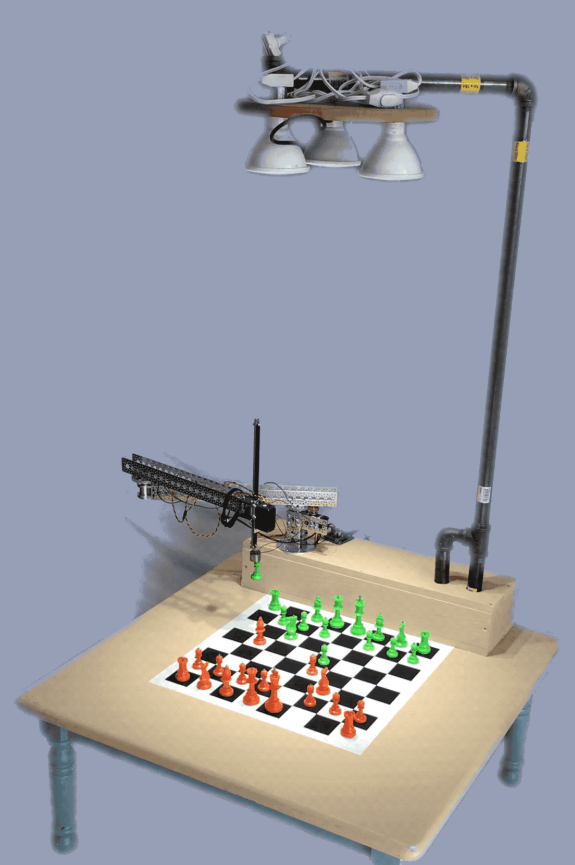
\includegraphics[width=0.8\linewidth]{02_Literature_study/figures/Turkhero.png}
  \caption{John Mayers version}
  \label{fig:sub1}
\end{subfigure}
\begin{subfigure}{.48\textwidth}
  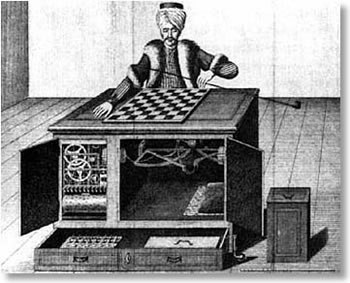
\includegraphics[width=1\linewidth]{02_Literature_study/figures/mechanical-turk.jpg}
  \caption{An illustration of the original Turk}
  \label{fig:sub2}
\end{subfigure}
\caption{The Mechanical Turk was a fake chess machine.}
\label{fig:test}
\end{figure}

\subsection{Chessboard sizes}
While the World Chess Federation (FIDE) has very strict rules \cite{FIDErules}when it comes to the physical size of the board and pieces, chess comes in all shapes and sizes commercially. According to FIDE the squares should be in the range of 5x5 cm to 6x6 cm. The diameter of the pawn piece is stated in FIDE's rulebook to be 50\% of the square sides. The kind is supposed to occupy 75\% of a square. 
\cite{roberti_francois}